\section{Race Weekend}

It's now the night before the first race - hopefully all the planning and preparations listed above are complete!

This section will chronologically walk through a hypothetical race weekend from Friday night before the first race,
through the end of the last race on Sunday afternoon.

For this example, there will be a criterium on Saturday,
and a team time trial (TTT) % TODO: put in glossary
and road race held on Sunday.

You will notice that roles shift as we transition from planning to the weekend operations -
in the previous planning sections, the \pbproleref{role:lead_org} was tasked with most work.
During the weekend, the \pbproleref{role:primary_promoter} will take the primary responsibility for the event.

A few example emergencies are included in this section, based on actual emergencies that have happened at previous ECCC races
(with some details changed for anonymity).
While we've attempted to include some unusual cases, keep in mind that emergencies may happen at any time, and can be highly unique and unusual.

\subsection{Friday Preparation}

The day before the criterium, the \pbproleref{role:lead_org} should ensure the crit course is swept and otherwise cleaned up,
either themselves or with assistance from \pbproleref{role:local_teams}.

Any no-parking signs, barriers, or other materials should be deployed (following the guidance and regulations of the local police and highway department).

The \pbproleref{role:lead_org} should have contracted a towing company to clear the crit course overnight.

\begin{marginfigure}
  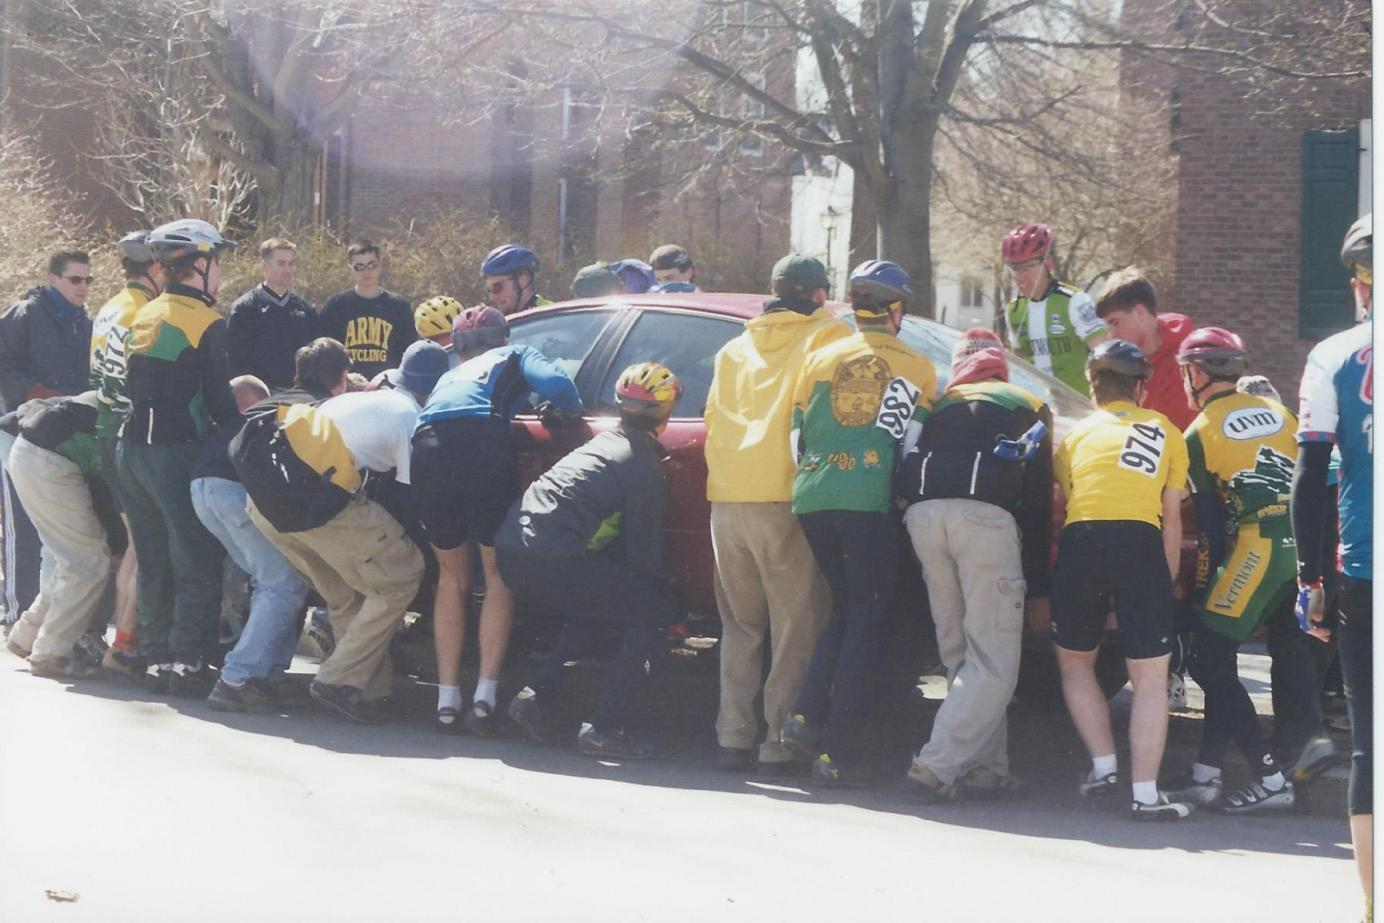
\includegraphics{dartmouth_car.jpg}
  \caption[Students moving a car off a criterium course]{
            Students moving a car off of the Darmouth criterium course
            when towing services were unavailable.\\
            Credit: Alan Atwood}
  \labfig{dartmouth_car}
\end{marginfigure}

The \pbproleref{role:primary_promoter} should call the towing company the night before the race to ensure they are still planning to clear the course -
otherwise you may have to resort to drastic measures (\reffig{dartmouth_car}) to clear the course in the morning!

\subsection{Friday Evening}

The \pbproleref{role:lead_org} and \pbproleref{role:primary_promoter} should ensure that race officials and staff are able to check in to their hotel rooms%
\sidenote{%
  You can pre-pay rooms at some hotels, so staff can just check-in by name and get a key.
  At other hotels, you may need to have an organizer check in with a credit card, and leave the keys for each person.}%
.

All traveling staff and cycling teams will trickle into the area throughout the night.
Given the large geographical size of the ECCC, people may be arriving quite late.

\subsection{Saturday Morning Setup}

The \pbproleref{role:primary_promoter} should plan to be the first person at the race, arriving at least two hours before the first race of the day
(\reffig{early_am_setup}).

\begin{marginfigure}
  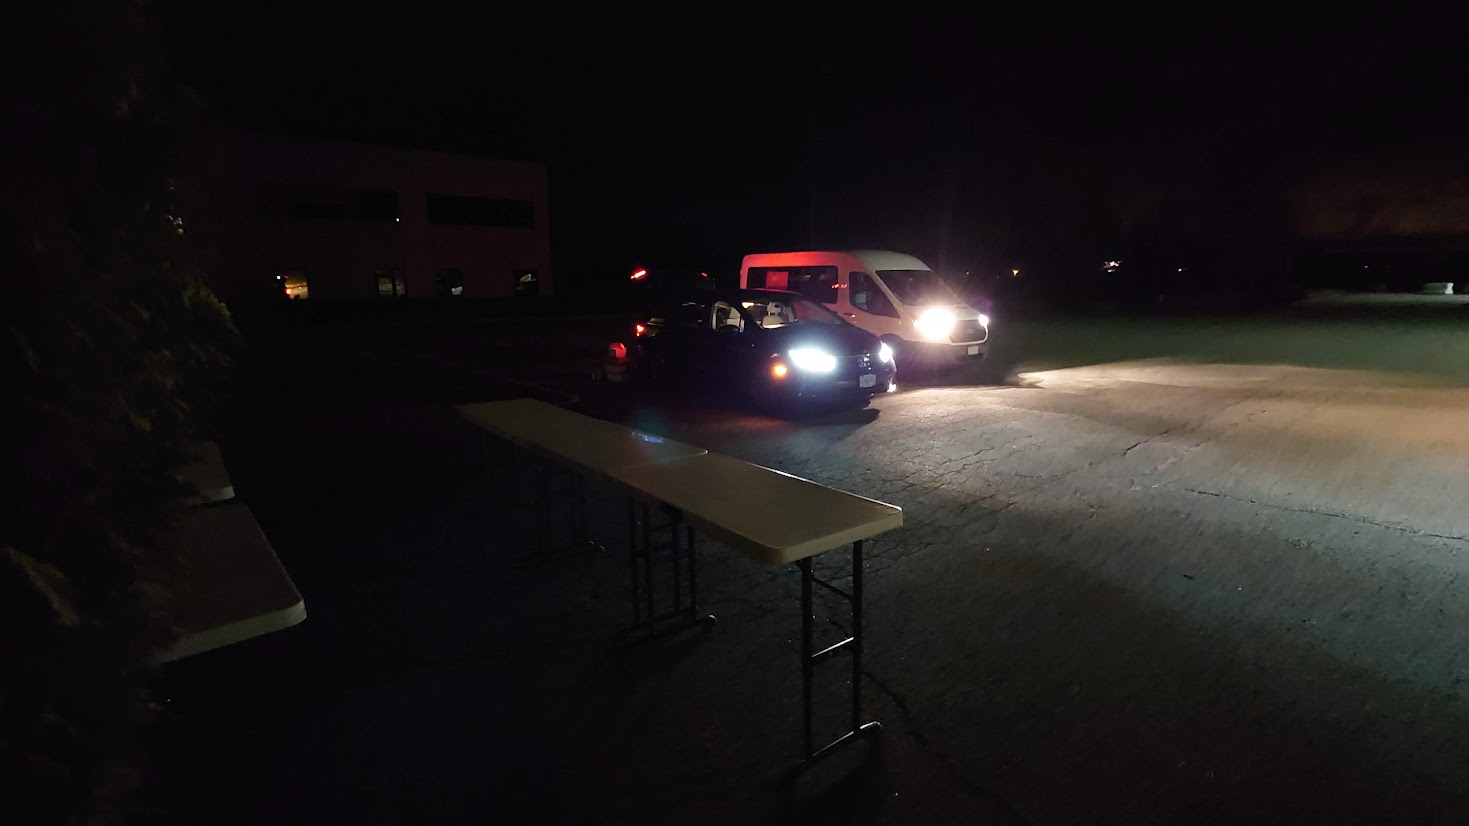
\includegraphics{2022_umass_early_am.jpg}
  \caption[Early morning race setup]{Expect to be setting up well before sunrise.\\
            Credit: Flyyn Leonard}
  \labfig{early_am_setup}
\end{marginfigure}

The \pbproleref{role:primary_promoter} should use this time to do a final check of the course,
ensuring that there are no hazards (sand on course, etc),
and that all directional signs and barriers are ready for the race.

If a location for the finish line has not been finalized, the \pbproleref{role:primary_promoter} should finalize that location now,
so the timing company, race officials, and riders can be informed of its location.

The \pbproleref{role:registrar} and \pbproleref{role:secondary_promoter} should be the next to arrive, at least 90 minutes before the first race of the day.

\subsubsection{Registration Setup}

The \pbproleref{role:registrar} should start setting up registration with assistance from the \pbproleref{role:primary_promoter} or \pbproleref{role:secondary_promoter}.

Registration must open 1 hour before the first race of the day, so setup is typically a high priority to ensure everything is ready before participants arrive.

\begin{itemize}
  \item Setup cover for registration - either hold registration inside or under the branded ECCC pop-up tent
  \item Ensure registration is locatable. If registration is under the branded ECCC tent that is typically sufficient, but if buildings block the view,
    ensure signs guide participants to registration
  \item Setup tables - typically a line of tables that participants approach, and additional tables at the back of the registration space
  \item Setup power
  \item Setup computers, printers, printers, the cash box
  \item Prepare supplies so they are easy to access: bib numbers, blank waivers, somewhere to store completed paperwork
\end{itemize}

\subsubsection{Volunteer Arrival}

The volunteer coordinator should ask that the first set of volunteers arrive between 60-90 minutes before the first race starts -
not so early that the volunteers disrupt the registration setup and first course sweep, but not too late that they need to be given directions
within the hectic hour before the first race.

\subsubsection{T-60 Minutes}

While the earlier hours are typically dark and quiet, everything starts to get busy one hour before the first race of the day starts.

Participants will start arriving in large numbers, needing help parking and directions to registration.
The \pbproleref{role:registrar} and any registration assistants will have their hands full processing registrations and handing out bib numbers,
and also being the point person that everyone asks for the day's schedule, which side to pin numbers on, and for directions to the bathrooms.

The timing company should arrive at least one hour before the first race.
The \pbproleref{role:primary_promoter} should greet them when they arrive,
and show them where the finish line is so the timing company can setup their equipment.

Race officials should be told to arrive one hour before the first race starts%
\sidenote{This is a USA Cycling standard.}.
The \pbproleref{role:primary_promoter} should meet the USA Cycling officials when they arrive,
The officials should be shown where everything is located, and the promoters should attend a briefing with the officials,
and ensure everyone is on the same page regarding communication (especially ensuring that race staff are not using a radio channel that the officials think is officials-only).

\subsubsection{T-30 Minutes}

Medical standby/EMTs should arrive around 30 minutes before the first race.
The \pbproleref{role:primary_promoter} should meet them when they arrive,
providing them with communication methods (radios, cell phone numbers), maps, and brief them on what the day will entail.

Police detail officers should also be arriving around 30 minutes before the first race.
The \pbproleref{role:primary_promoter} should meet and brief the officers, and ensure the officers block roads with barriers
before the race begins.
